\documentclass[tikz,border=10pt]{standalone}
\usetikzlibrary{arrows.meta,calc,decorations.pathreplacing}
\definecolor{green1}{RGB}{5, 168, 111}
\definecolor{faint1}{RGB}{59, 60, 54}
\definecolor{sunny}{RGB}{250, 211, 92} 


% ==== 5-BAR BATTERY SYMBOL (THIN BARS, AUTO RED, SCALABLE) ====
\newcommand{\battery}[2][0.32]{% #1 = scale (default 0.32), #2 = bar level
	\begin{tikzpicture}[scale=#1, thick]
		
		% --- COLOR RULE ---
		% Red for 1–2 bars, green otherwise
		\ifnum#2<3
		\def\barcolor{red!70!black}
		\else
		\def\barcolor{green!60!black}
		\fi
		
		% --- Battery Outer Case ---
		\draw[rounded corners=2pt] (0,0) rectangle (3.0,1.3);
		
		% --- Terminal ---
		\draw[rounded corners=1pt] (3.0,0.45) rectangle (3.3,0.85);
		
		% --- BAR WIDTH (thin bars) ---
		\def\bw{0.45}   % bar width
		\def\gap{0.10}  % gap between bars
		
		% --- DRAW 5 BARS, FILL ONLY UP TO LEVEL #2 ---
		% Bar 1
		\ifnum#2>0
		\fill[\barcolor] (0.15,0.15) rectangle (\bw+0.15,1.15);
		\fi
		% Bar 2
		\ifnum#2>1
		\fill[\barcolor] ({0.15 + (\bw+\gap)*1},0.15)
		rectangle ({0.15 + (\bw+\gap)*1 + \bw},1.15);
		\fi
		% Bar 3
		\ifnum#2>2
		\fill[\barcolor] ({0.15 + (\bw+\gap)*2},0.15)
		rectangle ({0.15 + (\bw+\gap)*2 + \bw},1.15);
		\fi
		% Bar 4
		\ifnum#2>3
		\fill[\barcolor] ({0.15 + (\bw+\gap)*3},0.15)
		rectangle ({0.15 + (\bw+\gap)*3 + \bw},1.15);
		\fi
		% Bar 5
		\ifnum#2>4
		\fill[\barcolor] ({0.15 + (\bw+\gap)*4},0.15)
		rectangle ({0.15 + (\bw+\gap)*4 + \bw},1.15);
		\fi
		
		% --- Optionally Draw Empty Bars (faint outline)
		\foreach \i in {0,1,2,3,4}{
			\draw[gray!60] ({0.15+(\bw+\gap)*\i},0.15) rectangle ({0.15+(\bw+\gap)*\i+\bw},1.15);
		}
		
	\end{tikzpicture}%
}



\begin{document}
	
	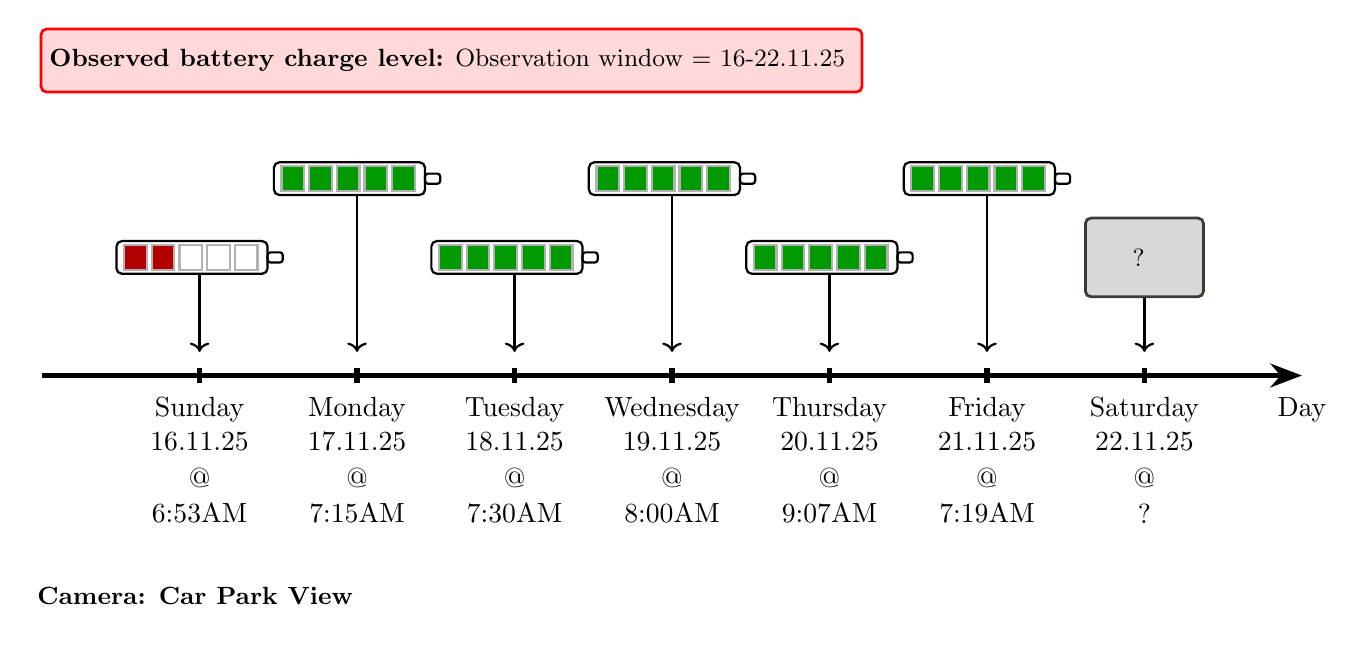
\begin{tikzpicture}[x=2cm, y=1cm, thick]
		
		% ---- MAIN TIMELINE ----
		\draw[-{Stealth[length=4mm,width=3mm]}, line width=2pt] (-1,0) -- (7,0);
		\node[below] at (7, -0.15) {Day};
		
		% ---- TICKS + YEAR LABELS ----
		\foreach \x/\day in {
			0/Sunday,
			1/Monday,
			2/Tuesday,
			3/Wednesday,
			4/Thursday,
			5/Friday,
			6/Saturday
		}
		{
			\draw[line width=2pt] (\x,0.1) -- (\x,-0.1);
			\node[below] at (\x,-0.15) {\day};
		}
		
		\foreach \x/\day in {
			0/16.11.25,
			1/17.11.25,
			2/18.11.25,
			3/19.11.25,
			4/20.11.25,
			5/21.11.25,
			6/22.11.25
		}
		{
			%\draw[line width=2pt] (\x,0.1) -- (\x,-0.1);
			\node[below] at (\x,-0.6) {\day};
		}
		
		\foreach \x/\day in {
			0/@,
			1/@,
			2/@,
			3/@,
			4/@,
			5/@,
			6/@
		}
		{
			%\draw[line width=2pt] (\x,0.1) -- (\x,-0.1);
			\node[below] at (\x,-1.05) {\day};
		}
		
		\foreach \x/\day in {
			0/6:53AM,
			1/7:15AM,
			2/7:30AM,
			3/8:00AM,
			4/9:07AM,
			5/7:19AM,
			6/ ?
		}
		{
			%\draw[line width=2pt] (\x,0.1) -- (\x,-0.1);
			\node[below] at (\x,-1.5) {\day};
		}
		
		
		% ======================================================
		% UNIFORM GAP ABOVE TIMELINE FOR ALL ARROWS
		% ======================================================
		\def\gapy{0.3}
		
		% ---- DIRECTED ARROWS ----
		\coordinate (a2004) at (0,1.3);   \draw[->, thick] (a2004) -- (0,\gapy);
		\coordinate (a2007) at (1,2.3);   \draw[->, thick] (a2007) -- (1,\gapy);
		\coordinate (a2011) at (2,1.3);   \draw[->, thick] (a2011) -- (2,\gapy);
		\coordinate (a2014) at (3,2.3);   \draw[->, thick] (a2014) -- (3,\gapy);
		\coordinate (a2017) at (4,1.3);   \draw[->, thick] (a2017) -- (4,\gapy);
		\coordinate (a2020) at (5,2.3);   \draw[->, thick] (a2020) -- (5,\gapy);
		\coordinate (a2023) at (6,1.5);   \draw[->, thick] (a2023) -- (6,\gapy);



		\node at (0,1.5) {\battery{2}}; % Sunday - 2 bars
		\node at (1,2.5) {\battery{5}}; % Monday - full
		\node at (2,1.5) {\battery{5}}; % Tuesday
		\node at (3,2.5) {\battery{5}};
		\node at (4,1.5) {\battery{5}};
		\node at (5,2.5) {\battery{5}};
		

\node[
		rectangle,
		draw=red,        
		fill=red!15,              
		minimum width=7cm,          
		minimum height=0.8cm,         
		rounded corners=2pt,        
		line width=1pt,
		align=center,                 
		inner sep=3pt, 
		anchor=center               
		] (box2004)
		at (1.6,4)                     
		{
				\small \textbf{Observed battery charge level:} Observation window = 16-22.11.25
				
		};
		
		
		\node[
		rectangle,
		draw=white,        
		fill=white,              
		minimum width=4cm,          
		minimum height=0.8cm,         
		rounded corners=2pt,        
		line width=1pt,
		align=center,                 
		inner sep=3pt, 
		anchor=center               
		] (box2004)
		at (0,-2.8)                     
		{
			\small \textbf{Camera: Car Park View}
			
		};
			




		
%		\node[
%		rectangle,
%		draw=green!40!black,        
%		fill=green!20,              
%		minimum width=3.5cm,          
%		minimum height=1cm,         
%		rounded corners=2pt,        
%		line width=1pt,
%		align=center,                 
%		inner sep=3pt, 
%		anchor=center               
%		] (box2004)
%		at (0,4)                     
%		{
%			\small Sustainable: 2004-2054\\
%			CBR = 16.00 \\
%			RROI = 2\% \\
%			Coverage $\uparrow$ = 3\%
%			
%		};
%		
%		\node[
%		rectangle,
%		draw=blue,        
%		fill=blue!20,              
%		minimum width=1.3cm,          
%		minimum height=0.9cm,         
%		rounded corners=2pt,        
%		line width=1pt,
%		align=center,                 
%		inner sep=3pt, 
%		anchor=center               
%		] (box2004)
%		at (1,1.5)                     
%		{
%			\small Reform Phase
%			
%		};
%		
%				
%		\node[
%		rectangle,
%		draw=red,        
%		fill=red!15,              
%		minimum width=9cm,          
%		minimum height=2.3cm,         
%		rounded corners=2pt,        
%		line width=1pt,
%		align=center,                 
%		inner sep=3pt, 
%		anchor=center               
%		] (box2004)
%		at (3.5,4)                     
%		{
%			\small \textbf{Scheme Not Financially Sustainable}, with Reserves \\ Projected to Deplete at Some Future Epoch ($T$) \\
%			\\
%			\\
%			
%		};
%		
%		\node[
%		rectangle,
%		draw=red!40,        
%		fill=sunny!20,              
%		minimum width=2cm,          
%		minimum height=1cm,         
%		rounded corners=2pt,        
%		line width=1pt,
%		align=center,                 
%		inner sep=3pt, 
%		anchor=center               
%		] (box2004)
%		at (1.85,3.5)                     
%		{
%			\footnotesize  CBR = 8.56 \\
%		\footnotesize	Eqbm = 2018
%			
%		};
%		
%		
%		\node[
%		rectangle,
%		draw=red!40,        
%		fill=sunny!20,              
%		minimum width=2cm,          
%		minimum height=0.5cm,         
%		rounded corners=2pt,        
%		line width=1pt,
%		align=center,                 
%		inner sep=3pt, 
%		anchor=center               
%		] (box2004)
%		at (2.95,3.26)                     
%		{
%			\footnotesize  CBR = 8.37 
%			
%			
%		};
%		
%		
%		\node[
%		rectangle,
%		draw=red!40,        
%		fill=sunny!20,              
%		minimum width=2cm,          
%		minimum height=0.5cm,         
%		rounded corners=2pt,        
%		line width=1pt,
%		align=center,                 
%		inner sep=3pt, 
%		anchor=center               
%		] (box2004)
%		at (4.05,3.26)                     
%		{
%			\footnotesize  CBR = 7.60 
%			
%			
%		};
%		
%		
%		\node[
%		rectangle,
%		draw=red!40,        
%		fill=sunny!20,              
%		minimum width=2cm,          
%		minimum height=1cm,         
%		rounded corners=2pt,        
%		line width=1pt,
%		align=center,                 
%		inner sep=3pt, 
%		anchor=center               
%		] (box2004)
%		at (5.15,3.5)                     
%		{
%			\footnotesize  CBR = 7.18 \\
%			\footnotesize	Eqbm = 2029
%			
%		};
%		
%		
%		
		\node[
		rectangle,
		draw=faint1,        
		fill=faint1!20,              
		minimum width=1.5cm,          
		minimum height=1cm,         
		rounded corners=2pt,        
		line width=1pt,
		align=center,                 
		inner sep=3pt, 
		anchor=center               
		] (box2004)
		at (6,1.5)                     
		{
			\small ?
			
			
		};
%		
		

		
		
		

	\end{tikzpicture}
	
\end{document}
